\documentclass[a4paper,landscape]{article}
\usepackage[margin=1cm]{geometry}
\usepackage{tikz}
\usepackage{xcolor}
\usepackage{amsmath}
\usetikzlibrary{mindmap, trees, shadows, positioning, arrows.meta, fit, backgrounds}

\definecolor{mathblue}{RGB}{30, 100, 200}
\definecolor{fmtgreen}{RGB}{30, 160, 80}
\definecolor{reasonorange}{RGB}{220, 120, 20}
\definecolor{penaltyred}{RGB}{190, 40, 40}
\definecolor{capviolet}{RGB}{120, 40, 180}
\definecolor{curriculumgray}{RGB}{60, 60, 60}
\definecolor{topcolor}{RGB}{20, 20, 20}
\definecolor{nodebg}{RGB}{245, 245, 250}

\pagestyle{empty}

\begin{document}

% ── Page 1: Overview ──────────────────────────────────────────────────────────
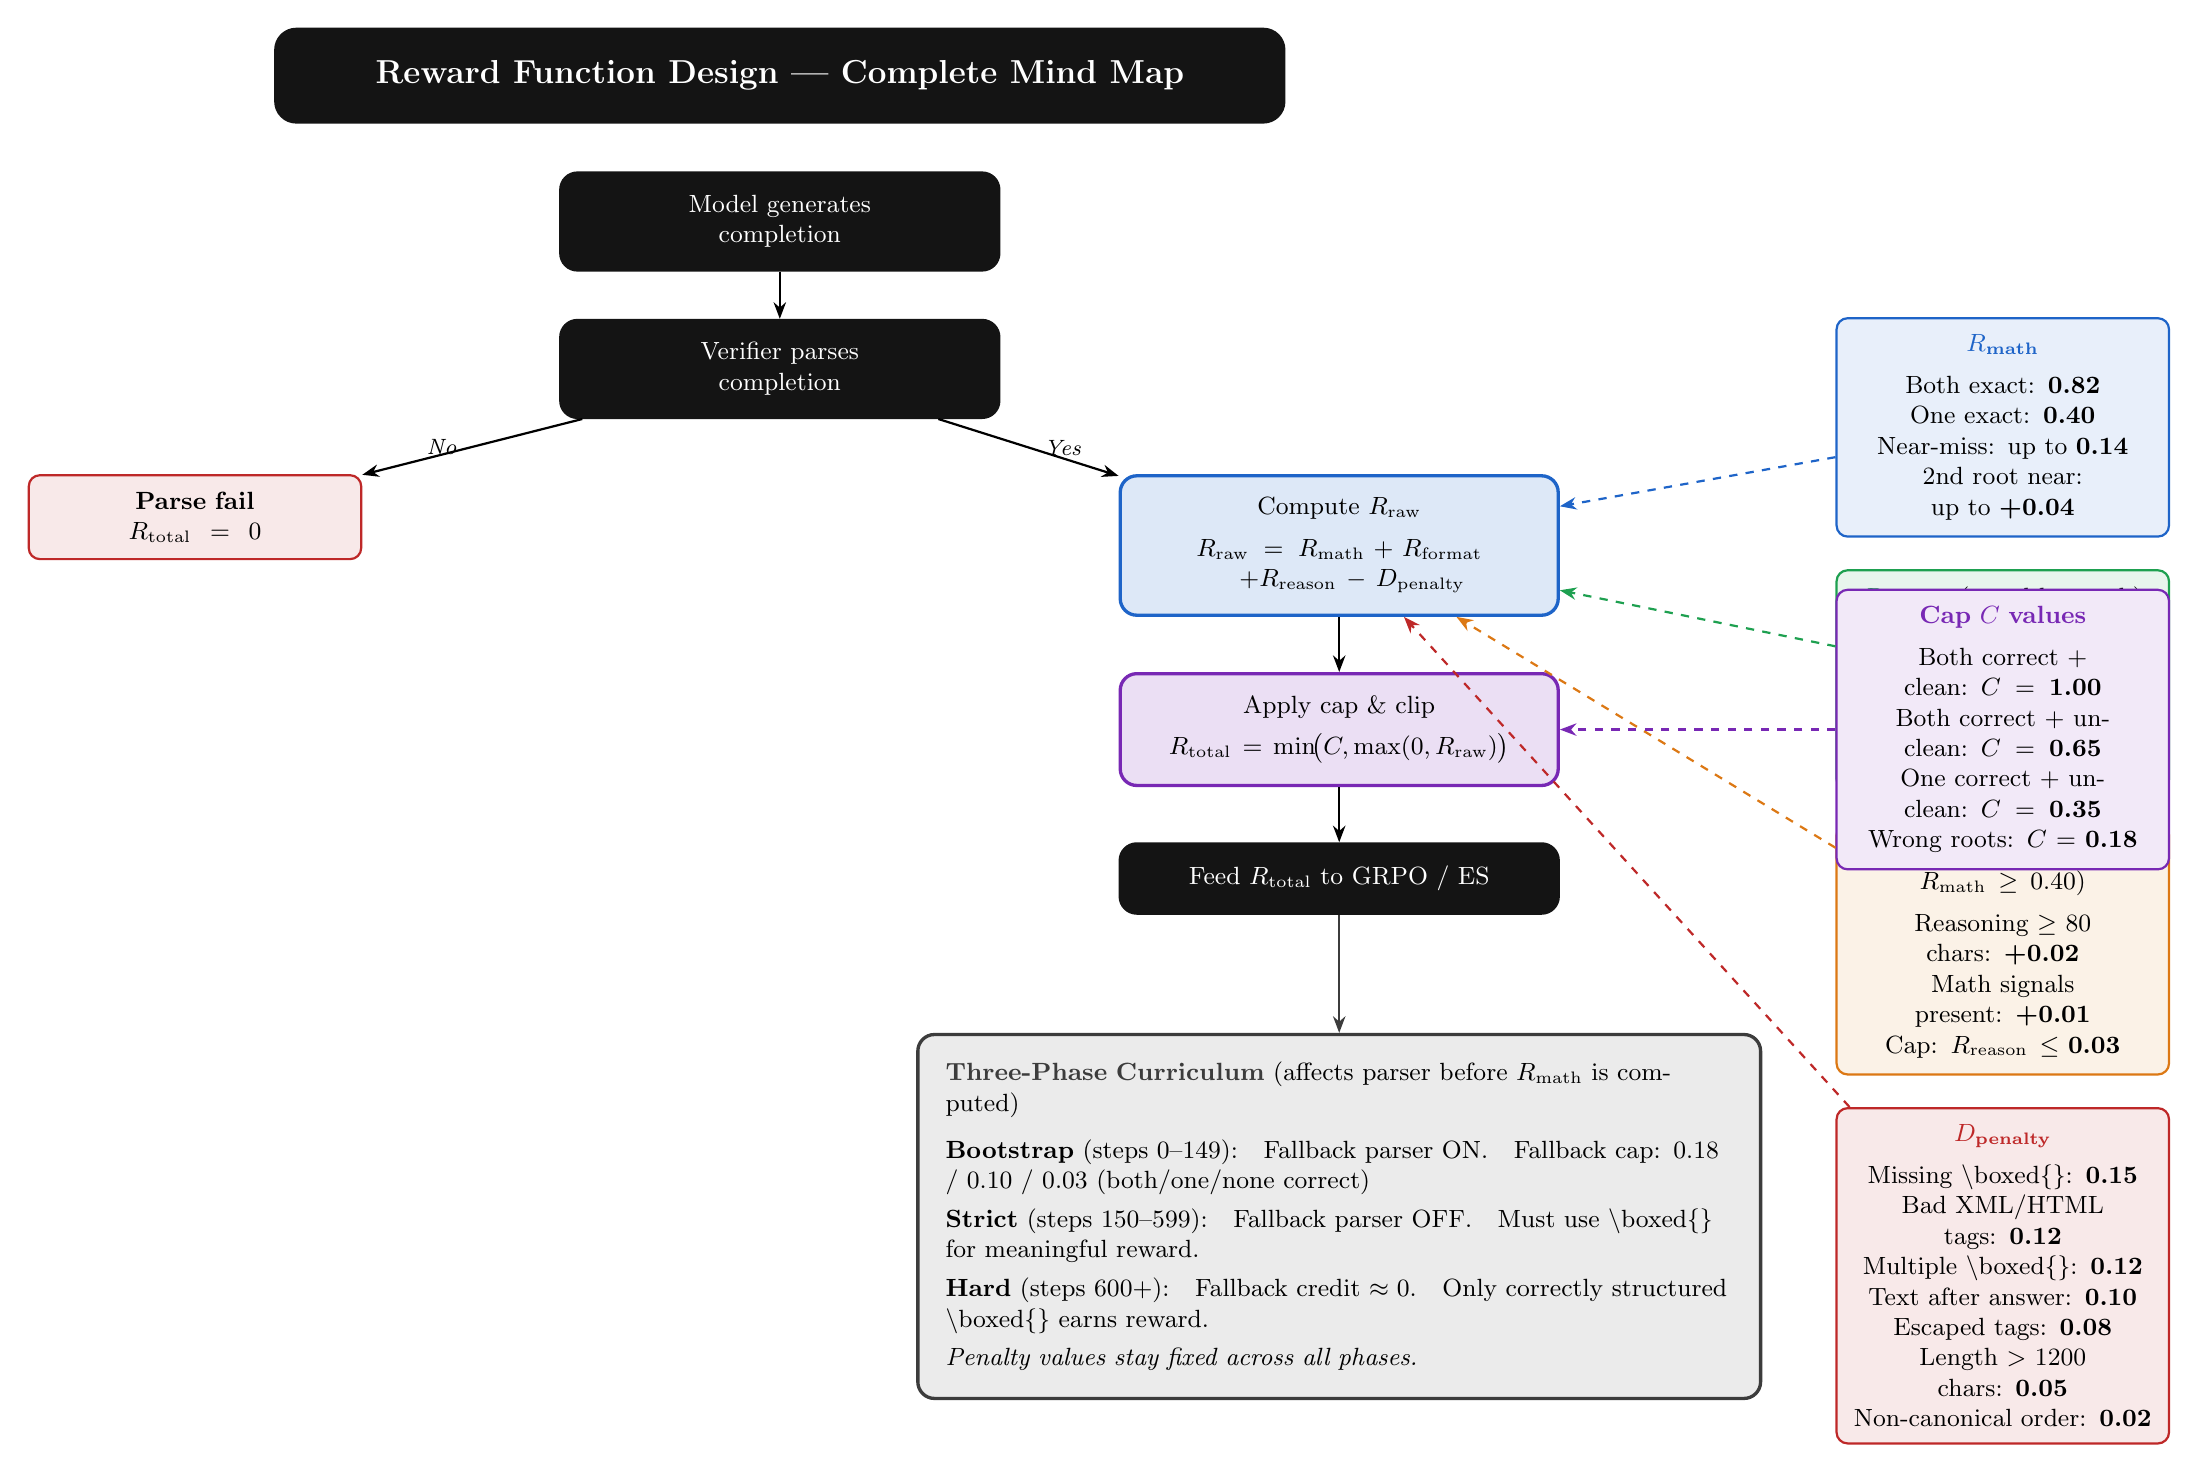
\begin{tikzpicture}[
  every node/.style={font=\small},
  box/.style={
    rectangle, rounded corners=4pt,
    draw=#1, fill=#1!10, thick,
    text width=3.8cm, align=center,
    inner sep=6pt
  },
  bigbox/.style={
    rectangle, rounded corners=6pt,
    draw=#1, fill=#1!15, very thick,
    text width=5.0cm, align=center,
    inner sep=8pt
  },
  arrow/.style={-{Stealth[length=6pt]}, thick, #1},
  label/.style={font=\footnotesize\itshape, #1}
]

% ── Title ─────────────────────────────────────────────────────────────────────
\node[rectangle, rounded corners=8pt, fill=topcolor, text=white,
      font=\large\bfseries, inner sep=12pt, text width=12cm, align=center]
  (title) at (0,0)
  {Reward Function Design --- Complete Mind Map};

% ── Top-level flow ────────────────────────────────────────────────────────────
\node[bigbox=topcolor, text=white, fill=topcolor, below=0.6cm of title]
  (gen) {Model generates\\completion};

\node[bigbox=topcolor, text=white, fill=topcolor, below=0.6cm of gen]
  (parse) {Verifier parses\\completion};

\node[box=penaltyred, below left=0.7cm and 2.5cm of parse]
  (nopars) {\textbf{Parse fail}\\$R_{\text{total}} = 0$};

\node[bigbox=mathblue, below right=0.7cm and 1.5cm of parse]
  (raw) {Compute $R_{\text{raw}}$\\[4pt]
         $R_{\text{raw}} = R_{\text{math}} + R_{\text{format}}$\\
         $\quad + R_{\text{reason}} - D_{\text{penalty}}$};

\node[bigbox=capviolet, below=0.7cm of raw]
  (cap) {Apply cap \& clip\\[4pt]
         $R_{\text{total}} = \min\!\bigl(C,\max(0, R_{\text{raw}})\bigr)$};

\node[bigbox=topcolor, text=white, fill=topcolor, below=0.7cm of cap]
  (opt) {Feed $R_{\text{total}}$ to GRPO / ES};

% arrows top flow
\draw[arrow=black] (gen) -- (parse);
\draw[arrow=black] (parse) -- node[label=black, left=2pt]{No} (nopars);
\draw[arrow=black] (parse) -- node[label=black, right=2pt]{Yes} (raw);
\draw[arrow=black] (raw)   -- (cap);
\draw[arrow=black] (cap)   -- (opt);

% ── R_math box ────────────────────────────────────────────────────────────────
\node[box=mathblue, right=3.5cm of raw, yshift=1.5cm]
  (rmath) {\textcolor{mathblue}{\textbf{$R_{\text{math}}$}}\\[4pt]
           Both exact: \textbf{0.82}\\
           One exact:  \textbf{0.40}\\
           Near-miss:  up to \textbf{0.14}\\
           2nd root near: up to \textbf{+0.04}};

% ── R_format box ──────────────────────────────────────────────────────────────
\node[box=fmtgreen, below=0.4cm of rmath]
  (rfmt) {\textcolor{fmtgreen}{\textbf{$R_{\text{format}}$}} (gated by math)\\[4pt]
          Both exact + clean: \textbf{0.15}\\
          Both exact + loose: \textbf{0.04}\\
          One exact  + clean: \textbf{0.06}\\
          One exact  + loose: \textbf{0.02}\\
          Wrong      + clean: \textbf{0.01}};

% ── R_reason box ──────────────────────────────────────────────────────────────
\node[box=reasonorange, below=0.4cm of rfmt]
  (rreason) {\textcolor{reasonorange}{\textbf{$R_{\text{reason}}$}} (only if $R_{\text{math}}\!\geq\!0.40$)\\[4pt]
             Reasoning $\geq$ 80 chars: \textbf{+0.02}\\
             Math signals present:      \textbf{+0.01}\\
             Cap: $R_{\text{reason}} \leq$ \textbf{0.03}};

% ── D_penalty box ─────────────────────────────────────────────────────────────
\node[box=penaltyred, below=0.4cm of rreason]
  (dpen) {\textcolor{penaltyred}{\textbf{$D_{\text{penalty}}$}}\\[4pt]
          Missing \textbackslash boxed\{\}: \textbf{0.15}\\
          Bad XML/HTML tags:       \textbf{0.12}\\
          Multiple \textbackslash boxed\{\}: \textbf{0.12}\\
          Text after answer:        \textbf{0.10}\\
          Escaped tags:             \textbf{0.08}\\
          Length $>$ 1200 chars:    \textbf{0.05}\\
          Non-canonical order:      \textbf{0.02}};

% ── Cap C box ─────────────────────────────────────────────────────────────────
\node[box=capviolet, right=3.5cm of cap]
  (cbox) {\textcolor{capviolet}{\textbf{Cap $C$ values}}\\[4pt]
          Both correct + clean:   $C=\textbf{1.00}$\\
          Both correct + unclean: $C=\textbf{0.65}$\\
          One correct  + unclean: $C=\textbf{0.35}$\\
          Wrong roots:            $C=\textbf{0.18}$};

% connecting arrows to R_raw
\draw[arrow=mathblue,   dashed] (rmath)   -- (raw);
\draw[arrow=fmtgreen,   dashed] (rfmt)    -- (raw);
\draw[arrow=reasonorange,dashed](rreason) -- (raw);
\draw[arrow=penaltyred, dashed] (dpen)    -- (raw);
\draw[arrow=capviolet,  dashed] (cbox)    -- (cap);

% ── Curriculum box ────────────────────────────────────────────────────────────
\node[rectangle, rounded corners=6pt,
      draw=curriculumgray, fill=curriculumgray!10, very thick,
      text width=10cm, align=left, inner sep=10pt,
      below=1.5cm of opt]
  (curr) {
    \textbf{\textcolor{curriculumgray}{Three-Phase Curriculum}}
    (affects parser before $R_{\text{math}}$ is computed)\\[6pt]
    \textbf{Bootstrap} (steps 0--149):\quad
      Fallback parser ON.\quad
      Fallback cap: 0.18 / 0.10 / 0.03 (both/one/none correct)\\[3pt]
    \textbf{Strict} (steps 150--599):\quad
      Fallback parser OFF.\quad
      Must use \textbackslash boxed\{\} for meaningful reward.\\[3pt]
    \textbf{Hard} (steps 600+):\quad
      Fallback credit $\approx 0$.\quad
      Only correctly structured \textbackslash boxed\{\} earns reward.\\[3pt]
    \textit{Penalty values stay fixed across all phases.}
  };

\draw[arrow=curriculumgray] (opt) -- (curr);

\end{tikzpicture}

\newpage

% ── Page 2: Worked Examples ───────────────────────────────────────────────────
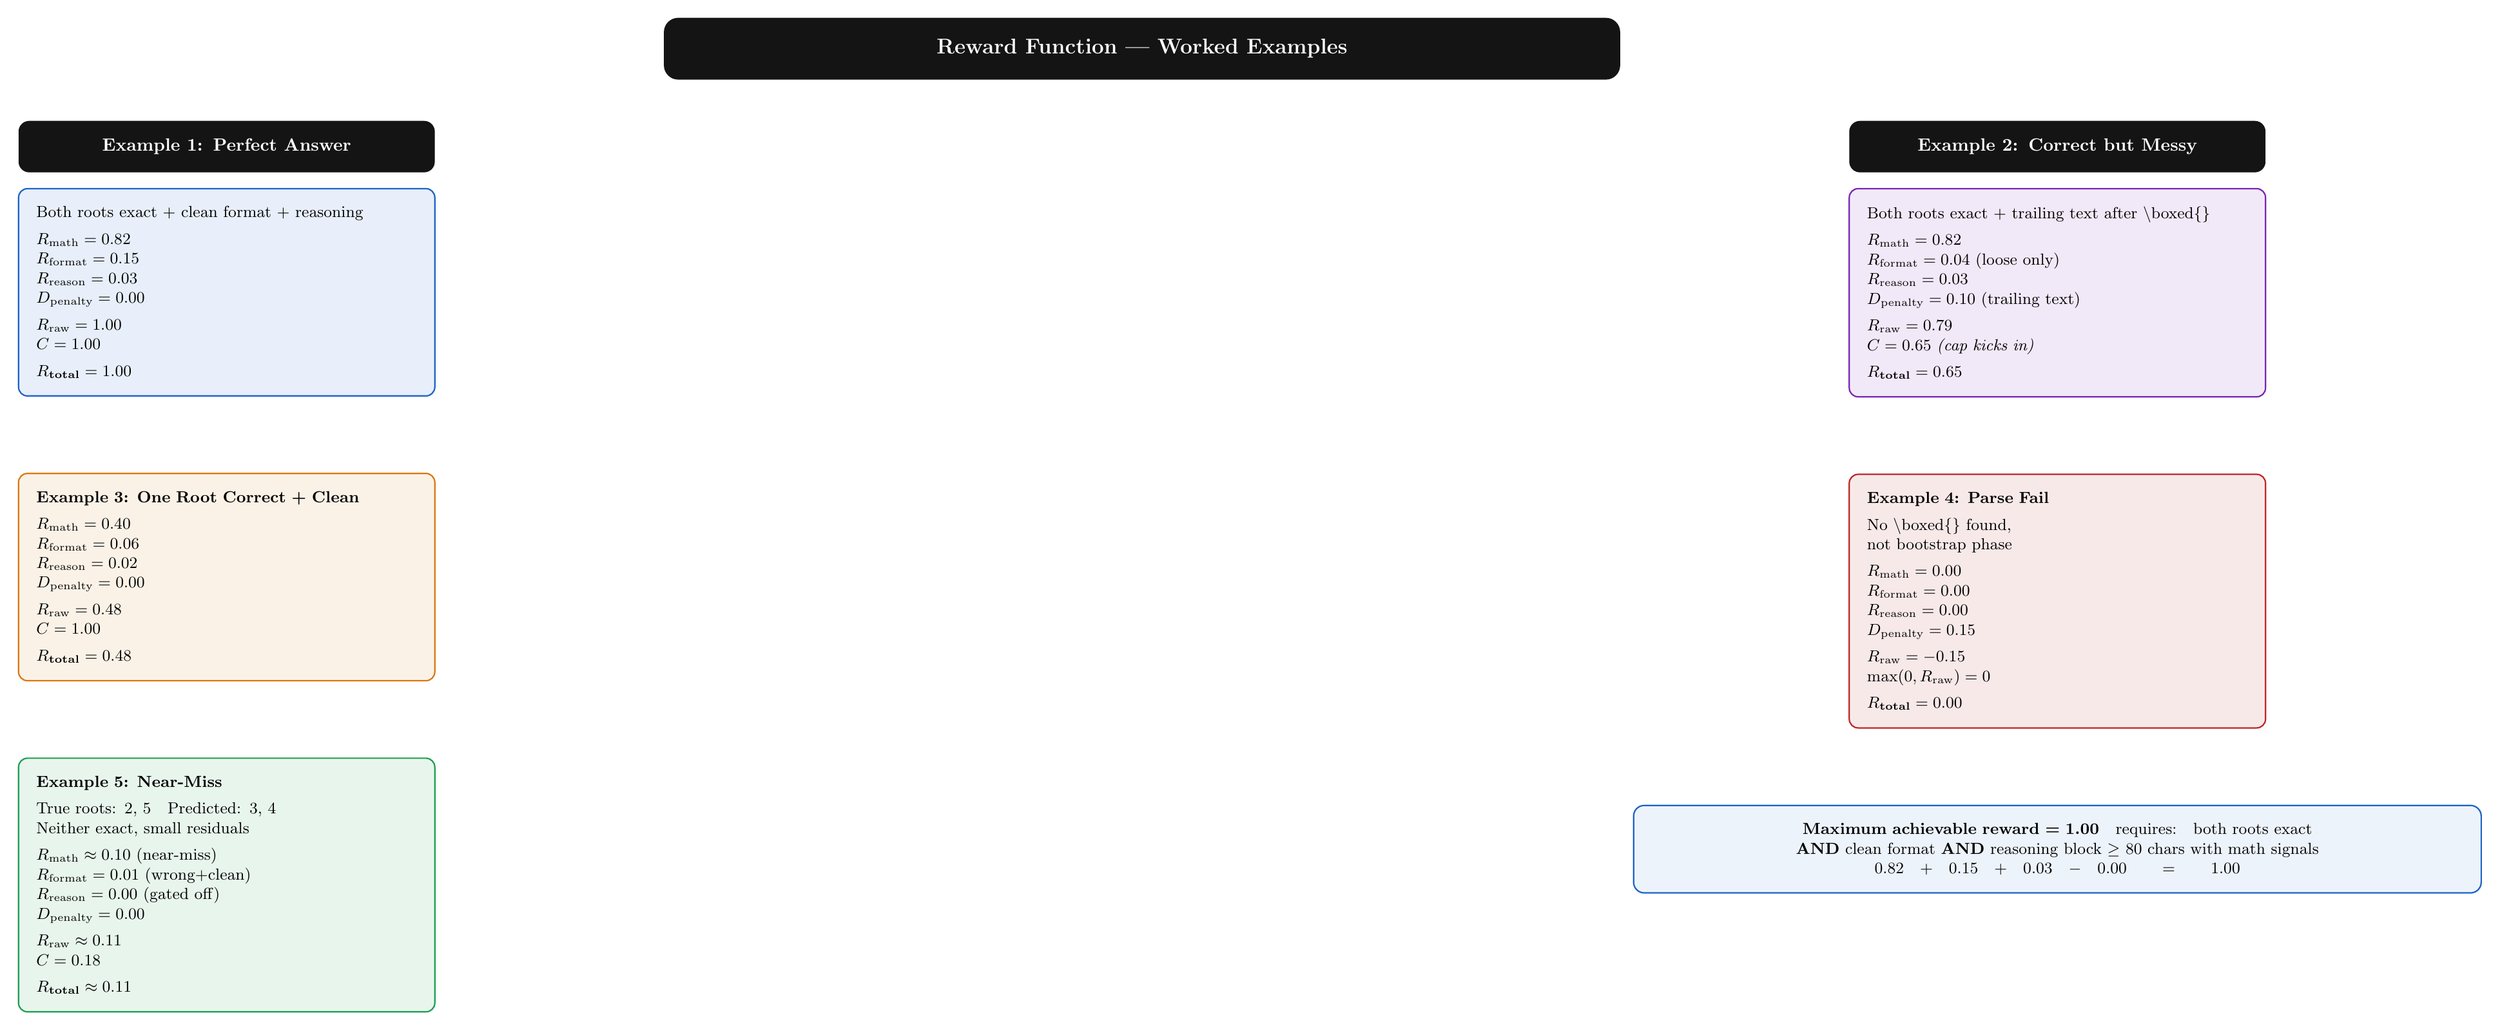
\begin{tikzpicture}[
  every node/.style={font=\small},
  exbox/.style={
    rectangle, rounded corners=5pt,
    draw=#1, fill=#1!10, thick,
    text width=7.5cm, align=left,
    inner sep=10pt
  },
  titlebox/.style={
    rectangle, rounded corners=6pt,
    fill=topcolor, text=white,
    font=\normalsize\bfseries,
    inner sep=10pt, text width=7.5cm, align=center
  }
]

\node[rectangle, rounded corners=8pt, fill=topcolor, text=white,
      font=\large\bfseries, inner sep=12pt, text width=18cm, align=center]
  (title2) at (0,0) {Reward Function --- Worked Examples};

% Example 1
\node[titlebox=topcolor, below left=0.8cm and 4.5cm of title2]
  (t1) {Example 1: Perfect Answer};
\node[exbox=mathblue, below=0.3cm of t1]
  (e1) {
    Both roots exact + clean format + reasoning\\[4pt]
    $R_{\text{math}}    = 0.82$\\
    $R_{\text{format}}  = 0.15$\\
    $R_{\text{reason}}  = 0.03$\\
    $D_{\text{penalty}} = 0.00$\\[4pt]
    $R_{\text{raw}}     = 1.00$\\
    $C                  = 1.00$\\[4pt]
    \textbf{$R_{\text{total}} = 1.00$}
  };

% Example 2
\node[titlebox=topcolor, below right=0.8cm and 4.5cm of title2]
  (t2) {Example 2: Correct but Messy};
\node[exbox=capviolet, below=0.3cm of t2]
  (e2) {
    Both roots exact + trailing text after \textbackslash boxed\{\}\\[4pt]
    $R_{\text{math}}    = 0.82$\\
    $R_{\text{format}}  = 0.04$ (loose only)\\
    $R_{\text{reason}}  = 0.03$\\
    $D_{\text{penalty}} = 0.10$ (trailing text)\\[4pt]
    $R_{\text{raw}}     = 0.79$\\
    $C                  = 0.65$ \textit{(cap kicks in)}\\[4pt]
    \textbf{$R_{\text{total}} = 0.65$}
  };

% Example 3
\node[exbox=reasonorange, below=1.5cm of e1]
  (e3) {
    \textbf{Example 3: One Root Correct + Clean}\\[4pt]
    $R_{\text{math}}    = 0.40$\\
    $R_{\text{format}}  = 0.06$\\
    $R_{\text{reason}}  = 0.02$\\
    $D_{\text{penalty}} = 0.00$\\[4pt]
    $R_{\text{raw}}     = 0.48$\\
    $C                  = 1.00$\\[4pt]
    \textbf{$R_{\text{total}} = 0.48$}
  };

% Example 4
\node[exbox=penaltyred, below=1.5cm of e2]
  (e4) {
    \textbf{Example 4: Parse Fail}\\[4pt]
    No \textbackslash boxed\{\} found,\\
    not bootstrap phase\\[4pt]
    $R_{\text{math}}    = 0.00$\\
    $R_{\text{format}}  = 0.00$\\
    $R_{\text{reason}}  = 0.00$\\
    $D_{\text{penalty}} = 0.15$\\[4pt]
    $R_{\text{raw}}     = -0.15$\\
    $\max(0, R_{\text{raw}}) = 0$\\[4pt]
    \textbf{$R_{\text{total}} = 0.00$}
  };

% Example 5 - near miss
\node[exbox=fmtgreen, below=1.5cm of e3]
  (e5) {
    \textbf{Example 5: Near-Miss}\\[4pt]
    True roots: 2, 5\quad Predicted: 3, 4\\
    Neither exact, small residuals\\[4pt]
    $R_{\text{math}}    \approx 0.10$ (near-miss)\\
    $R_{\text{format}}  = 0.01$ (wrong+clean)\\
    $R_{\text{reason}}  = 0.00$ (gated off)\\
    $D_{\text{penalty}} = 0.00$\\[4pt]
    $R_{\text{raw}}     \approx 0.11$\\
    $C                  = 0.18$\\[4pt]
    \textbf{$R_{\text{total}} \approx 0.11$}
  };

% Max reward note
\node[rectangle, rounded corners=6pt,
      draw=mathblue, fill=mathblue!8, thick,
      text width=16cm, align=center, inner sep=10pt,
      below=1.5cm of e4]
  (maxnote) {
    \textbf{Maximum achievable reward = 1.00}\quad
    requires:\quad
    both roots exact \textbf{AND} clean format \textbf{AND} reasoning block $\geq$ 80 chars with math signals\\
    $0.82 + 0.15 + 0.03 - 0.00 = 1.00$
  };

\end{tikzpicture}

\end{document}
